\thispagestyle{plain}
\chapter{Framework}
This chapter introduces the framework that was implemented to generate workloads, partition data and eventually benchmark a custom index that uses the partitioning.
\begin{figure}[H]
    \centering
    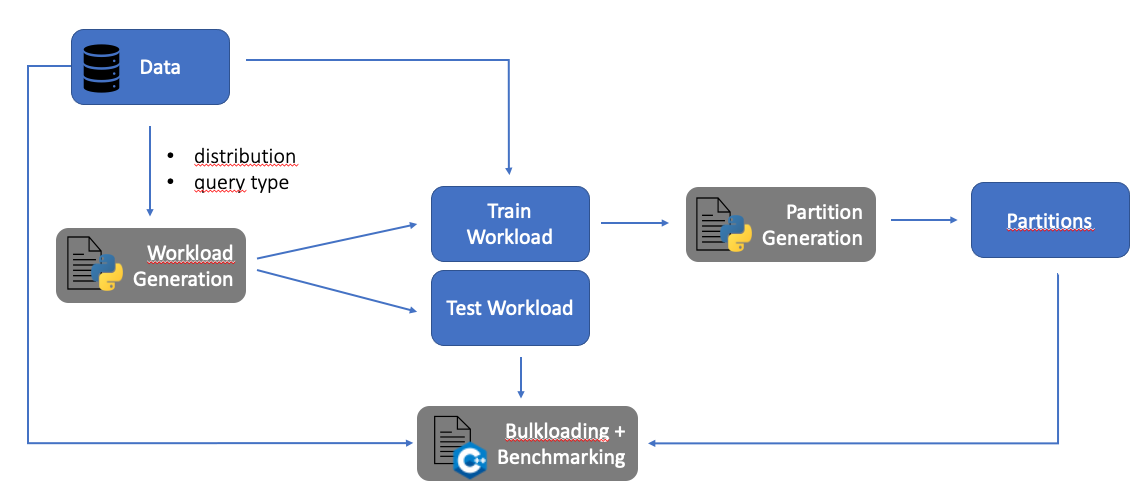
\includegraphics[width=\textwidth]{figures/pipeline.png}
    \caption{Framework Overview}
    \label{fig:framework}
\end{figure}

\section{Overview}
As we can see in Figure \ref{fig:framework}, the origin of all processes is the underlying data that should be indexed. Using a python script, we can specify properties like the distribution and type of queries (point, range) that should be generated to access the data through the index. The queries generated by this step are divided into a train and test workload and saved to files for later use in the C++ benchmarking.

TODO: Example of overlapping distributions

Given the train workload, the partitioning algorithms that are described in Sections \ref{sec:frequency} and \ref{sec:purity} can analyze the corresponding properties of the workload and will produce a partition of the underlying data. The resulting elements are saved to a file with additional information that can be used for the index construction.
With this partition, the index is bulkloaded from the data where each element of the partition corresponds to an individual leaf node. The additional information like relative frequency and predominant query type of a segment can be used to modify the index. For example, if only point queries access a segment, it could be beneficial to manage data access through a hash table instead of a normal B-tree leaf. The next step is to execute the test workload on the index and compare it to other state-of-the-art indexes that were introduced in Section \ref{sec:related_work}, namely a B$^+$-tree, an Adaptive Radix Tree (ART) and a Piecewise Geometric Model index (PGM).

\section{Workload Generation}
The ultimate goal of this work is to generate good partitions for the index construction like it was mentioned in Section \ref{bg:hybrid}. The inputs to the partitioning algorithms are therefore a dataset and a workload sample which we know is representative of the expected workload. However, for the purpose of evaluating and testing the algorithms and modifications later used, we were in need of a flexible way to generate workload data, especially since it proved hard to find available real-world workload data. The workload generation is done in a Python script specifying a series of \verb|Partition| objects that wrap the following information:

\begin{itemize}
    \item \verb|qtype|: The query type that should be generated in this section
    \item \verb|num|: The number of queries for this section
    \item \verb|distribution|: Distribution underlying the generated queries
    \item \verb|index|: Whether the generation happens index-based or domain-based
    \item \verb|min, max|: minimal and maximal values that indicate the section boundaries. Either index or domain-based, depending on the value of \verb|index|.
\end{itemize}

This gives us a very flexible way to generate arbitrary workloads. Note that while a partition generated for the index construction later satisfies that the elements are mutually disjoint, the \verb|Partition| objects used for workload generation do not need to be disjoint. This only means that we can overlap the boundaries of the objects to generate even more flexible workloads. In fact, it is the only way to generate regions of the data that are accessed through multiple types of queries, e.g.~ through both point and range queries. 

\section{Partitioning algorithms}
There are a plethora of properties that one could look at when analyzing query workloads, but inspired by the works in Section \ref{sec:related_work}, we decided to focus on two properties and look at how we could use these to partition the data and create segments. As described in the previous Section, we can use the train workload to partition the data. The test workload is immediately saved to file after creation and not seen by both partitioning algorithms. 

\subsection{Partitioning by Frequency} \label{sec:frequency}
The first algorithm analyzes the frequency of query access for each key in the key space. The motivation behind using the frequency as partition property is that hopefully we can benefit from caching effects during execution of the test workload. We would hope that highly frequent segments remain in cache so that subsequent queries can retrieve the location of the corresponding keys faster. Additionally, by analyzing the frequency, we can use that information to change the structure of the index. A first idea in this regard would be to shift highly frequent segments higher up in the tree, to prevent expensive pointer chasing when traversing the index.

We first realized, that key-by-key comparisons are not useful for a generalized partitioning algorithm because we can only operate on a train workload that is sampled from the general workload distribution. If we would use these key-by-key comparisons for the frequency to create partitions, we would probably overfit to the patterns in the train workload, even though these might only be caused by noise and not be present in the general distribution. Therefore, we employ an approach that tries to maximize the previously mentioned goal: find partitions where keys are accessed roughly the same amount of times. This partition should create elements, that utilize caching. Regions with almost no accesses will be put in one partition which will result in the segment being not loaded very often. On the other hand, regions with similarly frequent keys will result in the the corresponding segment remaining in cache if the frequency is high enough.

We use a single-pass algorithm that tries to find plateaus in the workload distribution by calculating the average change in frequency over a sliding window. It uses three phases depending on where it currently is with respect to a plateau, which are heavily inspired by the finite difference approximations from Section \ref{bg:numerical}:

\begin{enumerate}
    \item Start calculating a discrete forward difference approximation. As only keys "in the future" are considered, this phase is predestined to find an incoming plateau by checking if the calculated slope is near 0.
    \item After such a plateau was found, we use the central difference approximation to establish the boundaries of the plateau. We use this approximation now, as it considers keys from before and after the current one. This should give a better estimation of when a plateau is ending.
    \item Once the central approximation indicates that a plateau is ending, we switch to calculating the backward finite difference approximation to ensure that we find the exact end point of the plateau. We only consider previous keys, as we now know that an end is coming and this gives us the best chance to catch the key that is responsible for significantly changing the slope.
\end{enumerate}

//TODO: put algorithm code here

\subsection{Partitioning by Purity} \label{sec:purity}
\begin{itemize}
    \item Motivation: optimize index for different query types
    \item Algorithm
\end{itemize}

\section{Index Bulkloading and Benchmarking}
\subsection{Changing leaf data structure}
\subsection{Moving leaves higher up}
